\documentclass[a4paper]{article}

%% Language and font encodings
\usepackage[english]{babel}
%\usepackage[utf8x]{inputenc}
\usepackage[T1]{fontenc}
\usepackage{float}
\usepackage{subcaption}

%% Sets page size and margins
\usepackage[a4paper,top=3cm,bottom=2cm,left=3cm,right=3cm,marginparwidth=1.75cm]{geometry}

%% Useful packages
\usepackage{amsmath}
\usepackage{graphicx}
\usepackage{listings}
%\usepackage[colorinlistoftodos]{todonotes}
%\usepackage[colorlinks=true, allcolors=blue]{hyperref}

\title{Function-wise Execution Migration}
\author{Meet Udeshi}

\begin{document}
\maketitle

\section{Introduction}

Prior research has shown great potential of \textit{Heterogeneous-ISA chip multiprocessors} in terms of performance and energy gains. Implementation of such a processor involves one major challenge which is migrating execution of a process from one ISA to the other. Any implementation of such a system has to take care of \textit{Memory Image consistency} for both ISAs and perform necessary transformations during migration. The other main challenge is determining possible points of migration, and methods of identifying whether migration is beneficial, dynamically during runtime. To harness the benefits of ISA diversity fully, execution migration cost needs to be low enough so that frequent migration can be justified performance-wise.

\section{Memory Image consistency}

A program during execution accesses three different types of memory: Global, Stack and Heap.
Global memory is fixed at compile time hence can be maintained same for both ISAs. Heap memory grows during runtime and is only created according to a few functions like `malloc'. If implementation of these functions are same for both ISAs, then the image formed will be consistent \cite{execution-migration}. The stack memory is arranged by the compiler but it is created during runtime throughout execution of a function. The stack is very frequently accessed during runtime hence rearranging it for the purpose of image consistency would hit single threaded performance very hard.

The solution to this is to transform stack memory from layout created by one ISA to the layout expected by the other ISA. Stack transformation is the part which consumes the most time during execution migration.

\section{Migration Techniques}

To migrate entire process, we need to transform every stack frame individually and then update all pointers referring to stack memory with correct addresses. A standard implementation would require to wait for all stack frames to transform and then be able to migrate. This leads to a heavy cost of migration in the range of few 100 microseconds \cite{execution-migration}.

\subsection{Simultaneous Transformation}

\begin{figure}[H]
\centering
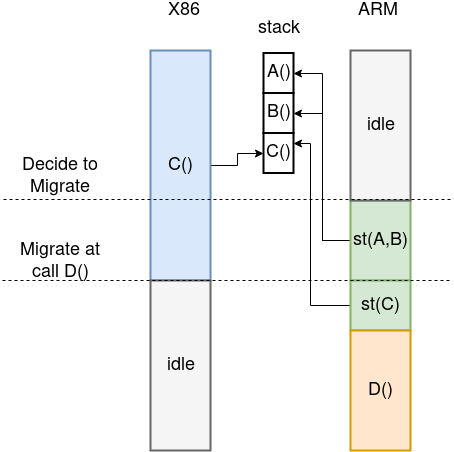
\includegraphics[width=0.3\textwidth]{simul_trans}
\caption{\label{fig:simul_trans}Simultaneous transformation of stack}
\end{figure}

When executing in function $C()$, previous frames in the stack are untouched by the program. This allows us to run stack transformation on those frames in parallel to program execution. This greatly reduces the time taken in stack transformation to time of transforming last function's frame.

\subsection{Single-frame transformation}

\begin{figure}[H]
\begin{subfigure}{0.5\textwidth}
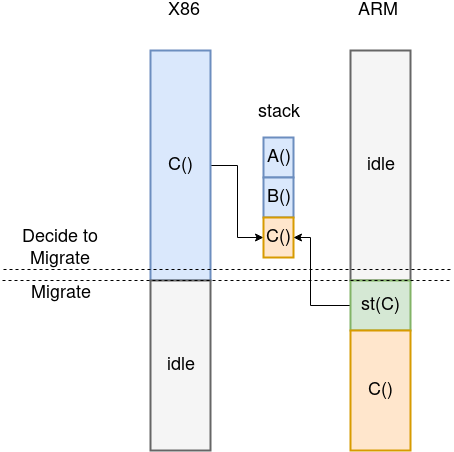
\includegraphics[width=0.8\textwidth]{singleframe_trans}
\caption{\label{fig:singleframe_trans}Single frame transformation of stack}
\end{subfigure}
\begin{subfigure}{0.5\textwidth}
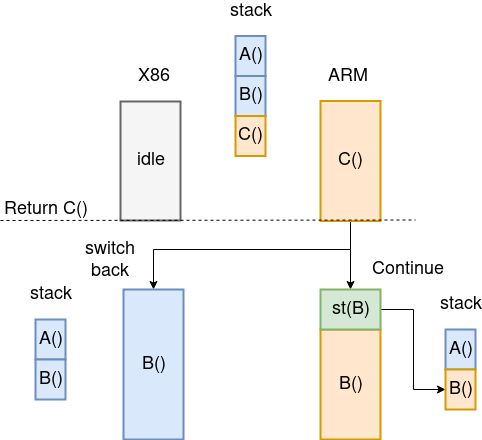
\includegraphics[width=0.8\textwidth]{singleframe_return}
\caption{\label{fig:singleframe_trans}Return from single frame transformed function}
\end{subfigure}
\end{figure}

Another alternate for reducing migration time is to only transform last function's stack when migrating. This allows us to harness the affinity of certain functions towards a specific ISA. When we feel that function currently executing would be affine to the other ISA, we migrate and only incur cost of transformation for the last stack frame. While returning, a decision is made to transform frame to current ISA, or switch back to previous ISA.

In worst case, we would have to transform every frame to new ISA when migrating one function. But that cost would be no worse than standard migration, which transforms all frames immediately.

\section{Implementation}

LLVM Compiler toolchain was used for stack and pointer analysis.
Internal steps for compiling using LLVM (\texttt{clang} compiler) are these:
\begin{itemize}
    \item Source code is converted to LLVM-IR by the Clang compiler.
    \item LLVM-IR is further processed by \texttt{llc} based on provided architecture parameters (Target triple)
    \item Generated object files for each source have to be linked to create single executable.
    \item The system linker is used, hence for ARM compilation on X86 host (cross-compile) we need to have an ARM compatible linker. One can use the package manager provided GCC cross-compiler linker without affecting any of the compilation steps by LLVM, provided only the linker is used.
\end{itemize}

\subsection{Stack frame map generation}

In generating a migration map for function stack, we require mapping of stack slots from X86 to ARM.
This mapping is found by looking at \texttt{alloca} statements at the start of function in LLVM-IR file.
The IR file is architecture independent, the variables assigned by \texttt{alloca} would hold the same data in both architectures.
We need to find the stack slot alloted to these variables and that will provide the required mapping.
Stack slot allocation happens in an \texttt{llc} pass called \texttt{prologepilog} which does Prolog-Epilog insertion
for each function. We take an output dump of Machine-IR code after this pass and look at the stack frame for the mapping.

\subsection{Migration sequence generation}

To save on time and memory-accesses during migration, we need to modify the stack inplace.
Inplace modification requires going in a sequence in which no data on the stack is overwritten.
\\
\\
As an example take function: \texttt{BZ2\_bzDecompressStream(bz\_stream*, int, int)}
\\
\\
\begin{minipage}[t]{0.5\textwidth}
\begin{tabular}{lccc}
\textbf{Slot} & \textbf{size} & \textbf{align} & \textbf{location} \\
\hline
X86: & & & \\
\hline
  \textit{fi.0} & 4 & 4 & [SP-28] \\
  \textit{fi.1} & 8 & 8 & [SP-24] \\
  \textit{fi.2} & 4 & 4 & [SP-36] \\
  \textit{fi.3} & 4 & 4 & [SP-32] \\
  \textit{fi.4} & 8 & 8 & [SP-16] \\
\hline
ARM: & & & \\
\hline
  \textit{fi.0} & 4 & 4 & [SP-20] \\
  \textit{fi.1} & 8 & 8 & [SP-32] \\
  \textit{fi.2} & 4 & 4 & [SP-36] \\
  \textit{fi.3} & 4 & 4 & [SP-40] \\
  \textit{fi.4} & 8 & 8 & [SP-48] \\
\end{tabular}
\end{minipage}
\begin{minipage}[t]{0.5\textwidth}
\centering
\begin{lstlisting}
tmp1 = frame[loc[1]]
frame[loc[1]] = frame[loc[0]]

for i=2..len(loc):
    tmp2 = frame[loc[i]]
    frame[loc[i]] = tmp1
    tmp1 = tmp2
\end{lstlisting}
\end{minipage}

When migrating from X86 to ARM, \texttt{fi.0} moves from location \texttt{[SP-28]} to \texttt{[SP-20]}.
Location \texttt{[SP-20]} already contains data of slot \texttt{fi.1} (\texttt{[SP-24]...[SP-17]}, size 8 bytes).
So we first have to backup \texttt{fi.1} locally and then overwrite with data from \texttt{fi.0}.
The locally stored \texttt{fi.1} will then be stored at its new location, after same backup procedure is applied.
This sequence will make sure migration is done inplace, and without loss or corruption of data.

The pseudo-code on the right lays out a method for migration using the sequence and two temporary variables.

\subsection{Pointer migration}

The previously generated LLVM-IR also helps us identify pointers to stack being created and passed to functions as arguments.
\texttt{alloca} instruction actually returns a pointer to the stack slot, which is stored in the SSA variable.
Generally when passing-by-value that variable is passed to a \texttt{load} instruction and data retreived is passed to the function arguments.
When the variable is used directly, that means that the function is getting passed a pointer of that stack-slot.
This is the case where we have to take care of migration i.e.
modifying the value of this pointer from X86 location to ARM location.
\\
\\
\begin{lstlisting}
define @functionA
  %2 = alloca i32
  %3 = alloca i64
    .
    .
  %51 = load i64, %3 i64*
  %52 = call @functionB(%51 i64, %2 i32*)
\end{lstlisting}

In the above example LLVM-IR code, \texttt{\%2} and \texttt{\%3} are pointers to two stack-slots.
As we can see, both are of type \texttt{i32*, i64*} respectively.
\texttt{\%3} is passed to the load function, hence the value of the stack-slot is now in \texttt{\%51} which is passed to the function.
However, \texttt{\%2} is passed directly to the function hence it is passed as a pointer.
We will have to take care of \texttt{functionB} when we migrate \texttt{functionA} because the value of pointer will need to be updated.
This has to be done for all functions where this pointer is passed to, directly or indirectly via multi-level calls.

\section{Simulation and Results}

We have used the LLVM+Clang toolchain for analysis of stack-frames of every function in the benchmark.
We have built tools to generate mapping of stack-slots in between X86 and AARCH64 ISAs.

We have implemented a stack-transformer currently as a C function \texttt{migrate()}, which can be called from inside the function at any point.
Running the benchmark in gem5 and timing the execution of \texttt{migrate()} function gives us the time taken for migration in both the methods shown above.

\begin{figure}[H]
\centering
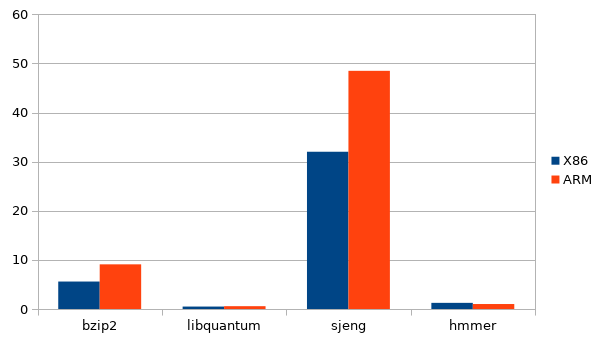
\includegraphics[width=0.7\textwidth]{avg_migration_time}
\caption{\label{fig:avg_migration_time}Migration time for various benchmarks}
\end{figure}

\end{document}
